\documentclass[10pt,twocolumn]{article}
\usepackage[margin=0.8in]{geometry}
\usepackage{booktabs,graphicx,amsmath,hyperref,xcolor}
% Placeholder for text / numbers that teammates still have to fill in (search for "\todo" in this file)
\newcommand{\todo}[1]{\textcolor{red}{[TODO: #1]}}
\title{AI6102 Team Project: Predicting Survival on the Titanic}
\author{%
  LIN, YUN-FAN (G2608301F) \and \todo{Member 2: NAME (Matric No.)} \and \todo{Member 3: NAME (Matric No.)}\\
}
\date{}
\begin{document}
\maketitle

\begin{abstract}
We study the Kaggle \emph{Titanic -- Machine Learning from Disaster} competition, a binary classification task.
We build a leakage-safe preprocessing and feature-engineering pipeline, compare several learning methods with repeated
stratified cross-validation, and analyse the contribution of each feature group with an ablation study.
A regularised logistic regression reaches $\approx$0.83 CV accuracy, on par with tree ensembles.
Adding fold-safe group-survival features raises the public score from 0.766 to 0.797.
\end{abstract}

\section{Problem Statement}
Given passenger records (class, name, sex, age, family aboard, ticket, fare, cabin, port of embarkation) predict whether a
passenger survived. The training set has 891 labelled passengers (38.4\% survived); the test set has 418 unlabelled ones.
Submissions are scored by accuracy on the hidden test labels.

\section{Challenges}
\begin{itemize}
  \item \textbf{Missing data:} Age is missing for 19.9\% of training rows, Cabin for 77.1\%, Embarked for 2 rows; the test set additionally lacks one Fare.
  \item \textbf{Small sample:} with 891 rows, CV estimates have a standard deviation of about 0.025, so small differences between methods are not significant.
  \item \textbf{Mixed, messy features:} free-text names, skewed fare, categorical codes, and strongly correlated variables (Sex/Title, Pclass/Fare/Cabin).
  \item \textbf{Overfitting risk} for flexible models on few samples.
\end{itemize}

\section{Proposed Solution}
\subsection{Motivation}
EDA shows that survival depends mainly on sex (74\% female vs.\ 19\% male), class (63\%/47\%/24\%), age (58\% for children)
and family size (non-monotonic). Cabin \emph{presence} is informative (67\% vs.\ 30\%).
We therefore (i) encode these signals explicitly as features, (ii) use a regularised linear model as the main method
(Occam's razor / structural risk minimisation), and (iii) compare against non-linear alternatives to check whether extra
complexity helps.

\subsection{Exploratory data analysis}
Fig.~\ref{fig:eda} summarises the survival rate of the main variables on the training set. Our reading of the plots drove every later design decision:
\begin{itemize}
  \item \textbf{Sex} is the strongest signal (74.2\% female vs.\ 18.9\% male), consistent with the ``women and children first'' rule. A sex-only rule already scores 0.787 on the training set.
  \item \textbf{Pclass} (a proxy for socio-economic status) is monotone: 63.0\%, 47.3\%, 24.2\% for classes 1, 2, 3.
  \item \textbf{Age} is non-linear: 58\% survival for ages $\le12$, about 40\% for adults, 23\% above 60. A single linear age term cannot express this, so we add a child indicator.
  \item \textbf{Family size} is non-monotone: passengers with 2--4 relatives survive most, those alone or in families of five or more survive least (SibSp$\ge$5: 0\%).
  \item \textbf{Fare} is strongly right-skewed (skewness 4.79; median 14.5, maximum 512), and survival increases with fare quartile (19.7\% $\to$ 58.1\%).
  \item \textbf{Missingness is informative:} passengers with a known cabin survive 66.7\% vs.\ 30.0\% without; 79\% of the missing ages belong to third-class passengers and 76\% to passengers travelling without relatives.
  \item Classes are mildly imbalanced (38.4\% positive), so we report F1 and AUC besides accuracy and use stratified folds.
\end{itemize}
\begin{figure*}[t]\centering
  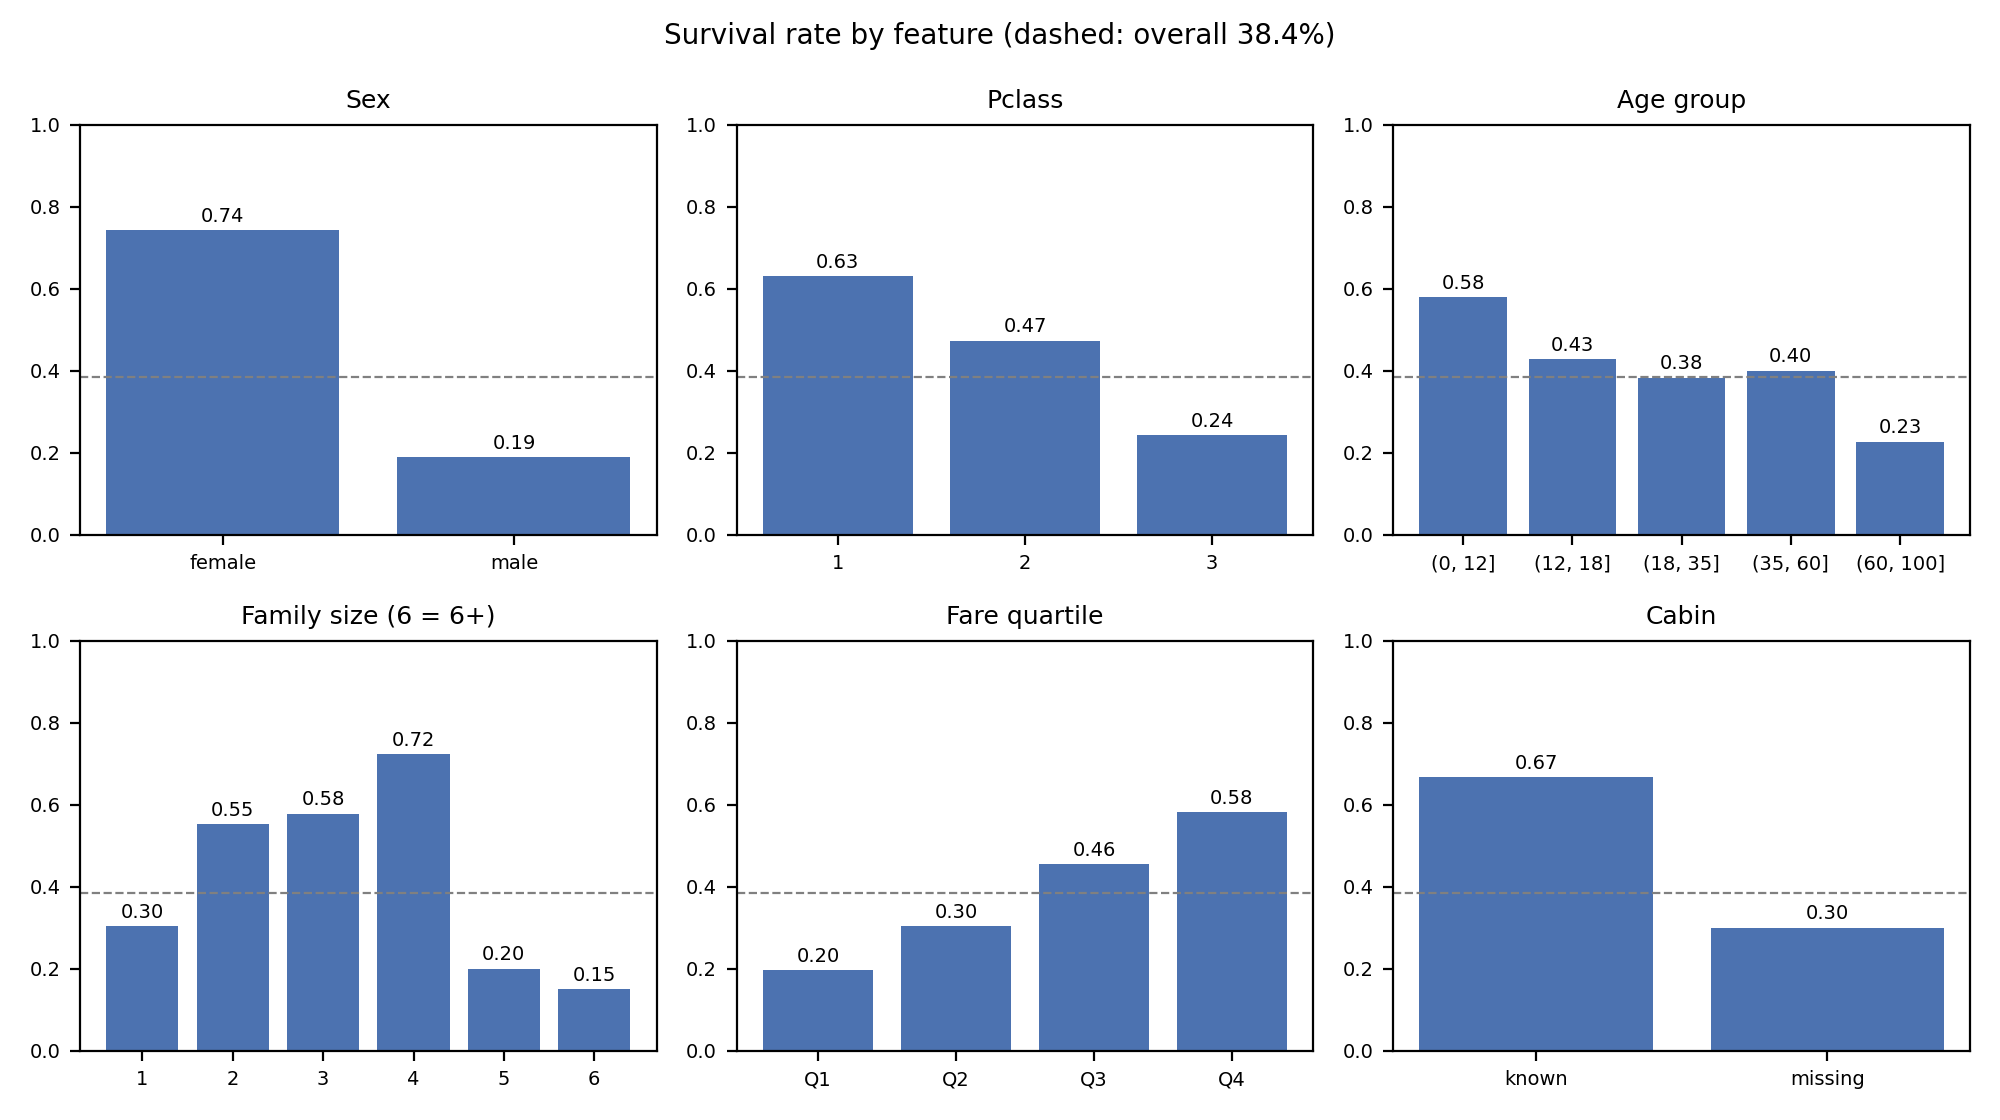
\includegraphics[width=0.85\textwidth]{eda.png}
  \caption{Survival rate by feature on the training set (dashed line: overall 38.4\%).}\label{fig:eda}
\end{figure*}

\subsection{Data preparation}
All statistics used for imputation come from the training data only and are applied unchanged to the test set.
\begin{table}[t]
\centering\small
\caption{Missing values and how they were handled.}
\label{tab:missing}
\begin{tabular}{p{1.0cm}p{1.2cm}p{4.6cm}}
\toprule
Column & Missing (train/test) & Treatment (reason) \\
\midrule
Age & 177 / 86 & Median age of the same Title$\times$Pclass$\times$[has Parch] group; flag \texttt{AgeMissing}. Titles separate boys (Master) from men and married from unmarried women, so this is more accurate than a global median (imputation MAE 8.2 vs.\ 11.2 years). \\
Embarked & 2 / 0 & Training mode (S); only two rows. \\
Fare & 0 / 1 & Median of the passenger's class (Fare is skewed; median is robust). \\
Cabin & 687 / 327 & Not imputed: 77\% missing, so any value would be fabricated. Missingness itself is informative, so it becomes \texttt{HasCabin}. \\
\bottomrule
\end{tabular}
\end{table}
No rows were removed (only 891 samples). Columns dropped: \texttt{PassengerId} (running index), \texttt{Name} (information extracted into Title and Surname), \texttt{Cabin} (replaced by HasCabin), \texttt{Ticket} (used only as a grouping key). Categorical variables (Title, Embarked, Pclass) are one-hot encoded because they are nominal and a linear model should not assume equal spacing; numeric variables are standardised inside the model pipeline.

\subsection{Feature engineering}\label{sec:fe}
Each feature is motivated by the EDA and validated by the ablation study (Sec.~\ref{sec:ablation}).
\begin{table*}[t]
\centering\small
\caption{Engineered features, definition and rationale.}
\label{tab:fe}
\begin{tabular}{p{2.6cm}p{6.5cm}p{7.2cm}}
\toprule
Feature & Definition & Rationale \\
\midrule
Title & Text between ``,'' and ``.'' in Name; Mlle/Ms$\to$Miss, Mme$\to$Mrs, other rare titles $\to$ Rare; one-hot. & Encodes sex, age group and marital status in one variable; also drives the age imputation. \\
Sex & female $=1$. & Strongest single signal. \\
Age, IsChild, AgeMissing & Imputed age; $\text{Age}<13$; missing indicator. & Child survival is a local effect that a linear age term cannot capture; missingness correlates with class. \\
Family flags & HasFamily ($\text{SibSp}+\text{Parch}>0$); HasChildren (adult with Parch$>0$); WithParents (minor with Parch$>0$); LargeFamily (size $\ge5$). & Survival is non-monotone in family size; flags are interpretable and removed the collinearity of SibSp, Parch and FamilySize. Without LargeFamily CV dropped by 1.7 points. \\
LogFare & $\log(1+\text{Fare})$. & Reduces skewness from 4.79 to 0.39 and raises the correlation with survival from 0.26 to 0.33; the $+1$ handles 15 free tickets. It stabilises the linear model but does not change CV accuracy. \\
HasCabin & Cabin not missing. & Proxy for deck / status. \\
TicketSize, FarePP & Passengers per ticket (counted on train+test, no labels); fare divided by ticket size. & A ticket is shared by a group, so fares are per group. \\
Group-survival rates & For every passenger: smoothed survival rate $(s+2\bar y)/(n+2)$ of the \emph{other} passengers with the same ticket / surname, their count, and the same rate restricted to women \& children and to adult men. & Relatives and travel companions tended to survive or die together. Largest single improvement (leaderboard 0.766$\to$0.797). \\
\bottomrule
\end{tabular}
\end{table*}
\paragraph{Avoiding leakage.} Group-survival features are derived from labels, so they are computed \emph{inside every CV training fold} using that fold's training labels only, with leave-one-out for the passenger's own row; test rows use all training labels. Imputation statistics and ticket counts use no labels. Scaling is fitted inside the pipeline of each fold.

\subsection{Logistic regression}
Our main model is $L_2$-regularised logistic regression (Lectures 3--4). For a feature vector $x$,
\[
p(y{=}1\mid x)=\sigma(w^\top x+b),\qquad \sigma(z)=\frac{1}{1+e^{-z}},
\]
and the parameters minimise the regularised cross-entropy, which equals the negative log-likelihood (MLE) plus a Gaussian prior:
\[
\min_{w,b}\ \tfrac12\|w\|_2^2 + C\sum_{i}\big[-y_i\log p_i-(1-y_i)\log(1-p_i)\big].
\]
This is structural risk minimisation: $1/C$ controls model complexity (Occam's razor). The objective is convex and differentiable, so a global optimum is found with L-BFGS (liblinear for $L_1$). Features are standardised so that the penalty treats all coefficients equally. We chose logistic regression because (i) the signals found in the EDA are largely additive, (ii) with 891 samples a low-variance model is preferable, and (iii) its coefficients can be interpreted: with standardised inputs the largest were LargeFamily ($-0.60$), Female ($+0.58$), Title\_Mr ($-0.54$), Title\_Master ($+0.42$), Title\_Mrs ($+0.38$), Age ($-0.31$), HasCabin ($+0.29$) and Pclass\_3 ($-0.27$). The regularisation strength $C$ is selected by cross-validation (Sec.~\ref{sec:reg}); other models serve as comparison.

\subsection{Evaluation protocol}
We use \textbf{stratified $5$-fold cross-validation repeated 5 or 10 times}; every candidate is evaluated on identical splits, so differences are paired. Hyper-parameters of $k$NN and SVM are tuned by \emph{nested} CV (inner 5-fold on each outer training fold). Metrics are accuracy, F1 and ROC-AUC. The Kaggle public score is used only as a final check. \textbf{Feature ablation:} we remove one feature group at a time (Sex, Pclass, Title, Age, Family, Fare, Cabin, Embarked), retrain with the same pipeline and splits, and report the change in accuracy and AUC relative to the full model; ``Only Sex'' gives the lower bound.

\textbf{Models compared.} Our own models: logistic regression ($L_2$ and $L_1$), logistic regression on PCA components, and random forest / gradient boosting as non-linear references. Teammates evaluate $k$NN, Gaussian Naive Bayes, decision tree and SVM with the same protocol (script \texttt{team\_experiment\_template.py}). All model comparisons, the regularisation sweep and the ablation use \textbf{dataset B} (23 label-free features, Sec.~\ref{sec:fe}); the group-survival features of dataset C enter only the iteration study of Sec.~\ref{sec:iter}.

\section{Experiments}
\subsection{Model comparison}
Table~\ref{tab:models} compares the methods on dataset B with repeated $5\times5$ CV (identical folds for everybody).
\begin{table}[t]
\centering\small
\caption{Repeated $5\times5$ stratified CV on dataset B (mean $\pm$ std of accuracy).}
\label{tab:models}
\begin{tabular}{lccc}
\toprule
Model & Accuracy & F1 & AUC \\
\midrule
Logistic Regression (L2, $C{=}0.1$) & 0.8296 $\pm$ 0.0215 & 0.7744 & 0.8717 \\
Logistic Regression (L1, $C{=}0.3$) & 0.8298 $\pm$ 0.0223 & 0.7732 & 0.8705 \\
Logistic Regression + PCA(10) & 0.8292 $\pm$ 0.0254 & 0.7725 & 0.8707 \\
Random Forest (reference) & 0.8312 $\pm$ 0.0169 & 0.7671 & 0.8799 \\
Gradient Boosting (reference) & 0.8292 $\pm$ 0.0233 & 0.7740 & 0.8762 \\
\midrule
$k$NN & \todo{fill} & \todo{fill} & \todo{fill} \\
Gaussian Naive Bayes & \todo{fill} & \todo{fill} & \todo{fill} \\
Decision Tree & \todo{fill} & \todo{fill} & \todo{fill} \\
SVM (linear / RBF) & \todo{fill} & \todo{fill} & \todo{fill} \\
\bottomrule
\end{tabular}
\end{table}

Logistic regression ($L_2$, $L_1$ and on PCA components) reaches 0.829--0.830, and the non-linear references random forest (0.831) and gradient boosting (0.829) are not better within one standard deviation (0.02): flexible models bring no accuracy gain over a regularised linear model on this data set, which supports our choice. The tree ensembles have a somewhat higher AUC (0.876--0.880 vs.\ 0.872), i.e.\ they rank passengers slightly better, but this does not translate into accuracy. Reducing the 23 features to 10 principal components loses nothing, so the one-hot features are redundant.
\todo{Members 2 and 3: after filling the last four rows of Table~\ref{tab:models}, add 3--5 sentences comparing $k$NN, Naive Bayes, decision tree and SVM with logistic regression (which assumptions fit / do not fit the data?).}

\subsection{Regularisation and over-fitting}\label{sec:reg}
Following the lecture on over-fitting and structural risk minimisation, we sweep $C$ (inverse regularisation strength) and compare training and validation accuracy (Table~\ref{tab:reg}).
\begin{table}[t]
\centering\small
\caption{Training vs.\ CV accuracy of $L_2$ logistic regression on dataset B (repeated $5\times5$ CV).}
\label{tab:reg}
\begin{tabular}{rccc}
\toprule
$C$ & Train & CV & Gap \\
\midrule
0.01 & 0.8334 & 0.8258 & 0.0076 \\
0.03 & 0.8359 & 0.8314 & 0.0045 \\
0.1 & 0.8357 & 0.8296 & 0.0061 \\
0.3 & 0.8352 & 0.8294 & 0.0058 \\
1 & 0.8355 & 0.8283 & 0.0072 \\
10 & 0.8359 & 0.8265 & 0.0094 \\
100 & 0.8358 & 0.8260 & 0.0098 \\
\bottomrule
\end{tabular}
\end{table}

For $C=0.01$ the model is slightly under-fitted (CV 0.826). For all $C\ge0.03$ the train--validation gap is below 1 point, so there is almost no over-fitting, and CV accuracy is highest at $C=0.03$ (0.831) and decreases slowly as regularisation is weakened ($C=100$: 0.826, gap 0.010), the typical onset of over-fitting. Following Occam's razor we prefer strong regularisation ($C\in[0.03,0.1]$) for equal performance. With $L_1$ regularisation only 12 (at $C=0.05$) to 14 (at $C=0.1$) of the 23 coefficients are non-zero while CV stays at 0.830--0.831, which shows that part of the feature set is redundant.

\subsection{Feature ablation}\label{sec:ablation}
Table~\ref{tab:ablation} shows the effect of removing one feature group at a time (logistic regression, dataset B).
\begin{table}[t]
\centering\small
\caption{Feature-group ablation, logistic regression ($L_2$, $C{=}0.1$) on dataset B, repeated $5\times5$ CV.}
\label{tab:ablation}
\begin{tabular}{lcccc}
\toprule
Setting & Acc & $\Delta$Acc & AUC & $\Delta$AUC \\
\midrule
All features & 0.8296 & +0.0000 & 0.8717 & +0.0000 \\
$-$ Sex & 0.8280 & -0.0016 & 0.8711 & -0.0007 \\
$-$ Pclass & 0.8294 & -0.0002 & 0.8699 & -0.0018 \\
$-$ Title & 0.8135 & -0.0162 & 0.8632 & -0.0085 \\
$-$ Age & 0.8271 & -0.0025 & 0.8727 & +0.0009 \\
$-$ Family flags & 0.8289 & -0.0007 & 0.8688 & -0.0029 \\
$-$ Fare & 0.8319 & +0.0022 & 0.8723 & +0.0005 \\
$-$ TicketSize & 0.8296 & -0.0000 & 0.8724 & +0.0007 \\
$-$ Cabin & 0.8269 & -0.0027 & 0.8710 & -0.0008 \\
$-$ Embarked & 0.8263 & -0.0034 & 0.8721 & +0.0003 \\
Only Sex & 0.7868 & -0.0429 & 0.7669 & -0.1049 \\
\bottomrule
\end{tabular}
\end{table}

\textbf{Title} is the only group whose removal clearly hurts (accuracy $-1.6$ points, AUC $-0.009$). Removing any other single group changes accuracy by less than 0.4 points, which is within the CV standard deviation (0.02); removing Fare even raises accuracy by 0.2 points. This does not mean the other groups are unimportant: they overlap. When the family flags \emph{and} the ticket-based features (TicketSize, LogFarePP) are removed together, accuracy drops by 1.6 points (0.8132, AUC 0.8627), whereas removing either set alone costs almost nothing (0.8289 and 0.8307): the two sets describe the same ``travelling in a group'' information. Likewise Title contains Sex: removing both Title and Sex gives 0.740, but removing only Sex gives 0.828, and Sex alone gives only 0.787 (AUC 0.767). A one-at-a-time ablation therefore underestimates groups that have a substitute; group-wise removal (as done here) is more informative than removing single columns, but the conclusions must be read together with these overlaps.

\subsection{Error analysis}
With $C=0.1$ the out-of-fold confusion matrix is TN$=477$, FP$=72$, FN$=83$, TP$=259$ (survivors: precision 0.782, recall 0.757, F1 0.770; non-survivors: recall 0.869). The model misses more survivors than it falsely flags; a lower decision threshold would trade precision for recall if detecting survivors were more important.

\subsection{Other methods}
\subsubsection{$k$-nearest neighbours (Member 2)}
\todo{Describe the method and why it may (not) fit the data; distance metric and feature scaling; tuned $k$ (nested CV); train-vs-CV curve over $k$; result row in Table~\ref{tab:models}.}
\subsubsection{Naive Bayes (Member 2)}
\todo{Describe the (Gaussian / Bernoulli) model and the independence assumption; discuss which of our features violate it (e.g.\ Sex and Title); result row in Table~\ref{tab:models}.}
\subsubsection{Decision tree (Member 3)}
\todo{Describe the splitting criterion; tune \texttt{max\_depth} / \texttt{min\_samples\_leaf} by nested CV; train-vs-CV curve over depth (over-fitting); show the tree or feature importances; result row in Table~\ref{tab:models}.}
\subsubsection{Support vector machine (Member 3)}
\todo{Linear vs.\ RBF kernel; tune $C$ (and $\gamma$) by nested CV; discuss margin / regularisation and the relation to logistic regression; result row in Table~\ref{tab:models}.}

\subsection{Iterative improvement and leaderboard}\label{sec:iter}
We iterated on features and models, always selecting with repeated stratified CV (identical folds for all candidates)
and recording the public leaderboard score of each submission (Table~\ref{tab:versions}).
\begin{table}[t]
\centering
\caption{Versions, CV accuracy (repeated stratified CV) and Kaggle public score (418 test passengers; one passenger $\approx 0.24$ points).}
\label{tab:versions}
\small
\begin{tabular}{p{3.9cm}cc}
\toprule
Version & CV acc. & Public score \\
\midrule
v1: basic features, LR (C=1) & 0.828 & 0.76555 \\
v2: + fold-safe group-survival features, soft-vote ensemble (LR, GB, RF) & 0.840 & \textbf{0.79665} \\
v3a: + women/children \& adult-men group rates, LR ($C{=}0.03$) & 0.844 & 0.78468 \\
v3b: same, ensemble & 0.844 & 0.78708 \\
v4a: simplified family flags, age imputed by Title$\times$Pclass$\times$HasParch, LR & 0.840 & 0.77990 \\
v4b: same, ensemble & 0.847 & 0.78947 \\
v5: gender rule + group-override rules (no learned parameters) & 0.847 & 0.79425 \\
v6: LR with RFE feature selection & 0.839 & 0.77990 \\
v6 avg.: majority vote (RFE-LR, ensemble, rule) & 0.847 & 0.79186 \\
vote5: majority vote of 5 submissions & --- & 0.79186 \\
\bottomrule
\end{tabular}
\end{table}
\paragraph{Key findings.}
(i) The only change that clearly helped was the group-survival information (same ticket / surname): $\approx$+1 point CV and $+0.03$ on the leaderboard (0.766 $\to$ $\approx$0.79).
(ii) Simplifying the family features (four flags instead of FamilySize/IsAlone/SibSp/Parch) kept CV unchanged once a ``large family'' flag was included (0.830 vs.\ 0.831) but removing it lost 1.7 points, because survival is non-monotone in family size.
(iii) Age imputation using family members' ages lowered the imputation MAE (8.61 $\to$ 8.10 years) but did not change survival accuracy; only 38--52 of the 263 passengers with missing age have a relative or ticket mate with a known age.
(iv) Feature selection (mutual information, RFE, L1; selected inside each fold) did not beat the full feature set (0.835--0.839 vs.\ 0.842), but the stable core was Sex, Title\_Mr/Mrs, Pclass\_3 and the ticket-group rates.
(v) Scores of v2--v6 span 0.780--0.797, i.e.\ 7 passengers. With 418 test passengers the standard error of an accuracy near 0.79 is $\approx 2$ points ($\approx 8$ passengers), so these versions cannot be statistically distinguished, and the CV ranking does not match the leaderboard ranking. We therefore treat CV as the primary model-selection criterion and the leaderboard only as a final check; we deliberately did not tune against the leaderboard.
% TODO: insert screenshot of the Kaggle leaderboard / submission list here (required by the instructions).
\begin{figure}[t]\centering
  % \includegraphics[width=\linewidth]{leaderboard.png}
  \fbox{\parbox{0.9\linewidth}{\centering Leaderboard screenshot (to be added)}}
  \caption{Kaggle leaderboard result.}
\end{figure}

\subsection{Why CV and leaderboard differ}
The training CV ($\approx$0.84) is higher than the public score ($\approx$0.79). Reasons: the test set is small (standard error $\approx$2 points); it is intrinsically harder (the sex-only rule scores 0.787 on train but 0.766 on test); imputation statistics were computed once on the full training set before CV (label-free, small effect); and in test, relatives who are also in the test set carry no known label, whereas group features in CV can use labels of relatives in the training folds.

\section{Conclusion}
Careful feature engineering (+4 points over a Sex/Pclass/Age baseline) mattered more than the choice of model: regularised
logistic regression, random forest and gradient boosting end within noise of each other. Title is the only single feature group
whose removal clearly hurts, and group-survival
(same ticket / surname) information gave the largest later improvement (leaderboard 0.766 $\to$ 0.797).
Beyond that, model complexity, feature selection and ensembling gave no distinguishable gains on this small data set.
Our final submission is v2 (public score 0.79665). \todo{Members 2 and 3: add one sentence on how $k$NN, Naive Bayes, decision tree and SVM compare.}
\textbf{Limitations:} the training set is small, CV differences are within one standard deviation, and the imputation
statistics were fitted once on the full training set before CV (label-free, so the optimistic bias is small, but a strict
pipeline would refit them inside each fold). \textbf{Future work:} ticket/surname group features, interaction terms, stacking.

\end{document}
